% Chapter 2

\chapter{Introduction} % Chapter title

\label{ch:introduction} % For referencing the chapter elsewhere, use \autoref{ch:examples} 

%----------------------------------------------------------------------------------------

\subsection{Chemistry and Catalysis}

\label{ss:chemistryandcatalysis}

\noindent The natural science of chemistry owes a great deal its origin of \textit{alchemy}---the ancient practice largely dedicated to the transmutation of matter (namely that of lead to gold), founded on the mystical beliefs in the Philosopher's Stone or the Universal Elixir. Many alchemical methods---including also the knowledge acquired from the purification of metals extracted from mining; the preparation of herb-based medicinal remedies; as well as the creation of jewelery---have led to many of the practical techniques in use today's chemistry labs. In fact, it was not until very recently, around the beginning of the seventeenth century, that chemistry began to emerge as a scientific discipline in the modern sense.\textsuperscript{\cite{greenberg:2007}}

With growing concerns regarding anthropogenic climate change, environmental pollution and the rapid depletion of fossil resources we as chemists have persuasive incentives to ensure that chemistry is carried out efficiently, sustainably and in a way that minimises the output of undesirable by-products. To achieve these goals, catalysis remains a key technology by reducing the waste output and energy required for chemical reactions to occur, whilst enabling reactions which would not be possible in their absence, whilst increasingi product selectivity and yield. Thus it is not surprising that catalysis is considered to be one of the twelve principles of green chemistry.\textsuperscript{\cite{anastas:1998}}

The power of catalysis has been recognised since ancient times and has in fact been utilised for the development and prosperity of mankind at least as far back as the Neolithic Revolution, ca. 12\,500 years ago. This transitional period marked a worldwide shift in many human cultures away from lifestyles revolving around hunting and gathering towards agriculture and settlement, which is more akin to the modern world. This cultural change led to the development of farming practices and led to the preservation of food supplies using microbes and their biological catalysts, known as enzymes.\textsuperscript{\cite{vogel:2019}}

The earliest evidence of enzyme-assisted brewing can be traced back even further to the Neolithic village of Jiahu in China around 7500 \spacedlowsmallcaps{BCE}, where investigators found early evidence of alcoholic beverages.\textsuperscript{\cite{mcgovern:2004}}

The Egyptians---who were well aware of early enzyme-assisted brewing techniques---also utilised microorganisms and malt to produce bread as far back as 2000$-$1200 \spacedlowsmallcaps{BCE}.\textsuperscript{\cite{samuel:1996}}

Of course mankind hasn't limited its enzyme technologies to just bread and beer. Material applications are indispensible and enzymes have proven advantageous here also. Starting from pigeon and/or dog dung it is possible to use the microbacterial enzymes in the softening of leather. As early as 7000$-$3300 \spacedlowsmallcaps{BCE} this was exploited for leather processing for all manner of tools including bags, boats, and shoes.\textsuperscript{\cite{possehl:1996}}

It was much later, in the begining of the twentieth century, that catalysis as a scientific field was established. Nobel prizes have been highlighted many of the most influential discoveries in this era. Friedrich Wilhelm Ostwald, who recieved a Nobel prize in 1907, was the first to identify the role of catalysts as accelerants of reactions without themselves being consumed in the process, as well as defining the principles of chemical equilibria. Paul Sabatier, subsequently won the Nobel prize winner in 1912 for demonstrating the hydrogenation of organic compounds using fine powdered metals---a synthetic method which remains highly relevant in today's synthetic toolbox.\textsuperscript{\cite{beller:2012}}

Undoubtedly, one of the greatest success stories in catalysis is the development of artificial nitrogen fixation, resulting from one of the world's most successful partnerships between the German chemists Fritz Haber and Carl Bosch. Once Haber demonstrated the catalytic generation of ammonia from nitrogen and hydrogen on benchtop scale, Bosch, who worked at \textit{Badische Anilin- und Soda-Fabrik} (BASF), was instrumental in developing the high pressure reaction vessels and scaling up the reaction to a viable industrial process. After rigorous, state-of-the-art experimentation, an iron catalyst developed by Mittasch,\textsuperscript{\cite{honkala:2005}} was successfully implemented for the generation of ammonia. The process, known now as the Haber--Bosch process, has facilitated the production of inorganic fertilisers and we no longer rely solely on \textit{Rhizobium} bacteria for biofixation of the nitrogen our bodies need to synthesise vital proteins. Ultimately this advancement led to a population boom in the twentieth century from just 1.6 billion in the year 1900 to six billion in 1999.\textsuperscript{\cite{smil:1999}} In fact some estimations indicate that more than half of the world's agricultural yield relies on the Haber--Bosch process, which continues to feed the world's growing population. The scientific community recognised the advancement by bestowing of two separate Nobel prizes in 1918 and 1931, to Haber and Bosch (with F. Bergius), respectively. 

In 1963, the Nobel prize in chemistry was awarded to Karl Ziegler and Giulio Natta for their chemical and technological discoveries which enable high polymers to be generated from $1$-alkene monomers. A plethora of highly versatile Ziegler--Natta catalysts have been used since the inception of the so-called first-generation in the early 1950s.\textsuperscript{\cite{nowlin:2010}} The industrial value of these findings have been tremendous and has led to the generation of some of the largest volume commodity chemicals on the planet. 

The 1970s saw the development in palladium-mediated cross-coupling reactions and in 2010 the Nobel prize in chemistry was shared between Richard F. Heck, Ei-Ichi Negishi, and Akira Suzuki \textit{for palladium-catalyzed cross couplings in organic synthesis}.\textsuperscript{\cite{nobel:2010}} Nowadays, the Suzuki--Miyaura reaction is the gold standard in biaryl coupling using homogeneous catalysis, and it has become ubiquitous in both academia and industry.

%a new field of chemistry was established, known as catalysis. Catalysis is a relatively new as a scientific discipline established its roots at the beginning of the twentieth century. Already for many years it was known that the addition of small quantities of a substance to a reaction mixture could vastly improve reaction rates and selctivities without itself being consumed in the process.\textsuperscript{\cite{beller:2012}}

% \noindent Growing concerns regarding anthropogenic climate change, environmental pollution and the rapid depletion of fossil resources are all powerful and persuasive incentives to ensure that chemistry is carried out efficiently, sustainably and in a way that minimises the output of undesirable by-products. Naturally, catalysis remains a key technology in this respect, by reducing the waste output and energy required for chemical reactions to occur, whilst enabling reactions which would not be possible in their absence, whilst increasingi product selectivity and yield. Thus it is not surprising that catalysis is considered to be one of the twelve principles of green chemistry.\textsuperscript{\cite{anastas:1998}}

Over time the very definition of a catalyst has evolved as our understanding of them has grown, but nowadays a catalyst is considered: \textit{a substance that increases the rate of a reaction without modifying the overall standard Gibbs energy change in the reaction}.\textsuperscript{\cite{iupac:2014}}

Catalysts by their very nature reduce the activation barrier (\textit{E}\textsubscript{a}) required for a reaction to occur and this is achieved by providing an alternative mechanism for the reactants to follow.

Nowadays ca. 85\% of all industrial chemical processes involve at least one catalytic step. This is a reflection of their abilities in accelerating transformations, promoting selectivity, and reducing waste output and energy consumption. Whilst for many decades rare and precious second and third row transition metals have been at the forefront of catalysis, today's state-of-the-art catalysts are increasingly dependent on the talents of Earth-abundant 3d-metals.\textsuperscript{\cite{hapke:2020}}

\subsection{Homogeneous vs. Heterogeneous Catalysis}

Catalysts can be divided into two main categories: \textit{homogeneous} catalysts and \textit{heterogeneous} catalysts. The main distinction is the relative physical states of the catalyst and the reacion mixture; in homogeneous catalysis the catalyst is in the same phase as the rest of the reaction mixture, whereas in heterogeneous catalysis the catalyst is in a different phase from the rest of the reaction mixture. In most cases a homogeneous catalyst is dissolved in a solution of reagents, and a heterogeneous catalyst is a solid which is insoluble in solution.

Both classes of catalysts have their advantages and disadvantages (summarised in Table \ref{tab:comparison}).

Heterogeneous catalysts are widely utilised in the chemical industry than homogeneous catalysts. One of the main reasons for this is the ease of separation of the catalyst (normally a solid) from reaction mixtures.

\begin{table}[h!]
\centering
\caption[General Differences Between Homogeneous and Heterogeneous Catalysts]{General Differences Between Homogeneous and Heterogeneous Catalysts}
\begin{tabular}{ c c }
\toprule
homogeneous & heterogeneous \\
\midrule
 well-defined active site & many possible active sites \\
 high selectivity & low selectivity \\
 difficult separation & facile separation \\
 react at low temperature & react at high temperature \\
\bottomrule
\end{tabular}
\label{tab:comparison}
\end{table}

\section{Copper}

Copper, with the symbol Cu and atomic number $29$ is positioned in the the $3$d-block of the periodic table between nickel and zinc. It is a naturally occuring trace element (\ie\, comprises $<0.1$ mg kg$^{-1}$ of the earth's crust) found in rocks and minerals and plays an important biochemical role as an essential micronutrient and for facilitating metabolic processes in both prokaryotes and eukaryotes.\textsuperscript{\cite{flemming:1989}}

Copper's capabilities in redox catalysis are well documented, and is widely utilised in nature in the metal centres of at least $25$ biological enzymes. Myriad oxidation processes are facilitated by copper-containing enzymes, including: cytochrome c oxidase, superoxide dismutase, amine oxidase, lysyl oxidase, dopamine $\beta$-hydroxylase, peptidylglycine $\alpha$-amidating monooxygenase, tyronsinase, galactose oxidase, hemocyanin, ceruloplasmin, laccase, and acorbate oxidase. What's more, each of these enzymes relies on molecular oxygen as the oxidant.\textsuperscript{\cite{tishchenko:2016}}

\section{Manganese}

Manganese, with the symbol Mn and atomic number 25, is positioned in the the 3d-block of the Periodic table between chromium and iron. It is the twelfth most abundant element in the Earth's crust,\textsuperscript{\cite{costa:2014}} and it's known for its remarkable ability to exist in many oxidation states which range from $-3$ to $+7$, of which $+2$, $+3$, $+4$, $+6$, and $+7$ are most common.

Mn was not recognised as an element until 1774 when German$-$Swedish chemist, Carl Wilhelm Scheele, analysed pyrolusite (MnO$_2$) and recognised the that the ore and its extracts contained a previously undiscovered element! However, it wasn't until Scheele supplied Johan Gottlieb Gahn, a Swedish chemist and metallurgist, with pyrolusite that elemental manganese was first extracted later that year.\textsuperscript{\cite{kemmitt:1973}} 

Despite appearing silver$-$grey in its pure metallic form, given its propensity towards oxidation, it's found in Nature in oxidised forms, such as the ores pyrolusite, romanechite, manganite, hausmannite, and rhodochrosite, etc. 

Mn is an element essential for all life on Earth and it takes an active role in metabolism of amino acids, lipids, proteins and carbohydrates. In fact it's encountered in myriad animal systems, including those responsible for immunity, reproduction, blood sugar regulation, and bone growth.\textsuperscript{\cite{banci:2012}}

Plants also rely on Mn to facilitate photosynthesis---the process which generates the very oxygen we breathe---by forming the metalloenzyme core within the chloroplasts.\textsuperscript{\cite{banci:2012}}

Despite its ubiquity in terrestrial life, some guidance regarding limits of consumption of Mn are given by the U.\,S. National Research Council (NRC); It has provided an \textit{\textbf{e}stimated \textbf{s}afe and \textbf{ad}equate \textbf{d}ietary \textbf{i}ntake} (ESADDI), which recommends adults consume between 2$-$5 mg day$^{-1}$ of Mn.\textsuperscript{\cite{banci:2012}}

In fact, overexposure to Mn can be highly damaging towards human health. Manganism (Mn poisoning) was first observed in 1837 by James Couper, who documented the neurological damage of five Scottish men who were suffering after grinding manganese dioxide. Chronic exposure to Mn only proliferated therafter as Mn became increasingly ubiquitary in the steel alloy industry. Fortunately, exposure to the levels of Mn detailed by Couper are rare. Nevertheless, concerns regarding its impact on human health are valid.\textsuperscript{\cite{costa:2014}}

For a comprehensive peer-reviewed toxicological overview, see the U.\,S. Agency for Toxic Substances and Disease Registry's 2012 report.\textsuperscript{\cite{williams:2012}} Therein the authors quote \textit{adequate intakes} of 2.3 mg day$^{-1}$ and 1.8 mg day$^{-1}$ for men and women, respectively, based on data sourced from the U.\,S. Institute of Medicine Food and Nutrition Board.\textsuperscript{\cite{trumbo:2001}}

\section{Iron}

Iron, with the symbol Fe and atomic number $26$ is positioned in the the $3$d-block of the Mendeleev table between manganese and cobalt. Despite being the most abundandant element on Earth (by mass), it constitutes just ca. $5$\% of the Earth's crust, making it the the fourth most abundant element therein.\textsuperscript{\cite{nicholls:1973}}

Metallic iron is rarely found in the earth's crust, occuring much almost always in an oxidised form, and thus mankind has been extracting Fe from ores as far back as ca. $1200$ \spacedlowsmallcaps{BCE}. Oxides and carbonates, such as \textit{magnetite} (Fe$_3$O$_4$), \textit{hematite} (Fe$_2$O$_3$) and \textit{siderite} (FeCO$_3$), constitute the most common ores of iron. Besides those, are sulfur- and silicate-based ores, including \textit{pyrite} (FeS$_2$) and \textit{silicate perovskite} (FeSiO).\textsuperscript{\cite{nicholls:1973}}

Iron is ferromagnetic, and has a Curie point (the temperature at which certain magnetic materials undergo a sharp change in their magnetic properties) of $768^{\circ}$C, at which point it undergoes an endothermic transformation to its paramagnetic form.\textsuperscript{\cite{nicholls:1973}} From the perspective of catalysis, iron has properties which make it a distinguished adversary in the field of homogeneous catalysis. Iron has a wide breadth of formal oxidation states which range from $-2$ to $+6$.\textsuperscript{\cite{fuerstner:2016}}

Biologically speaking, iron is an essential element for much of the animal life on Earth, playing an important role in the blood of most vertebrates. It binds readily with porphyrin-derived ligands to form, most notably, the oxygen-transport metalloproteins haemoglobin and myoglobin.

Iron has been used extensively in organometallic chemistry and catalysis. Famously it was utilised by German--Jewish chemist, Peter Pauson, and his student, Thomas J. Kealy, to create \textit{ferrocene}---the first known sandwich complex. Regrettably, both failed to identify the correct structure of the complex, and it wasn't until $1952$ that three groups (including Robert Burns Woodward) independently deduced the correct $\eta^{5}$ hapticity of the iron metallocene.

\section{Cobalt}

Cobalt, with the symbol Co and atomic number 27, is positioned in the 3d-block of the Mendeleev table between iron and nickel. It derived its name in medieval times from the German word \textit{Kobold} meaning Goblin, due to its resemblance to the more sought-after silver$-$copper ores mined in this era, but wasn't recognised as a discrete element until 1735 by Swedish chemist Georg Brand.

Cobalt has a d\textsuperscript{9} electron configuration and readily achieves formal oxidation states ranging from $-$1 to $+$3. In catalytic transformations it has a clear tendency towards the $+$1/$+$3 oxidation states, much like its noble neighbours, rhodium and iridium.\textsuperscript{\cite{hapke:2020}}

The demand for cobalt is intense in today's technological society as consumers rely increasingly on devices integrating rechargable batteries, including mobile phones, laptops, and increasingly, electric vehicles.\textsuperscript{\cite{crundwell:2011}}

The copper$-$cobalt mines in the Central Africa Copperbelt in the Democratic Republic of the Congo (DRC) (such as the much-publicised Mutanda Mine, shown in figure \ref{fig:mutanda}) and Zambia account for more than two thirds of the world's cobalt production, much of which is obtained as a by-product of coper and nickel extraction. It is found in sulfide ores (ca. 25\%), laterite ores (ca. 25\%)...\textsuperscript{\cite{crundwell:2011, wef:2020}}

\begin{figure}
\centering
\begin{minipage}{\textwidth}
   \centering
   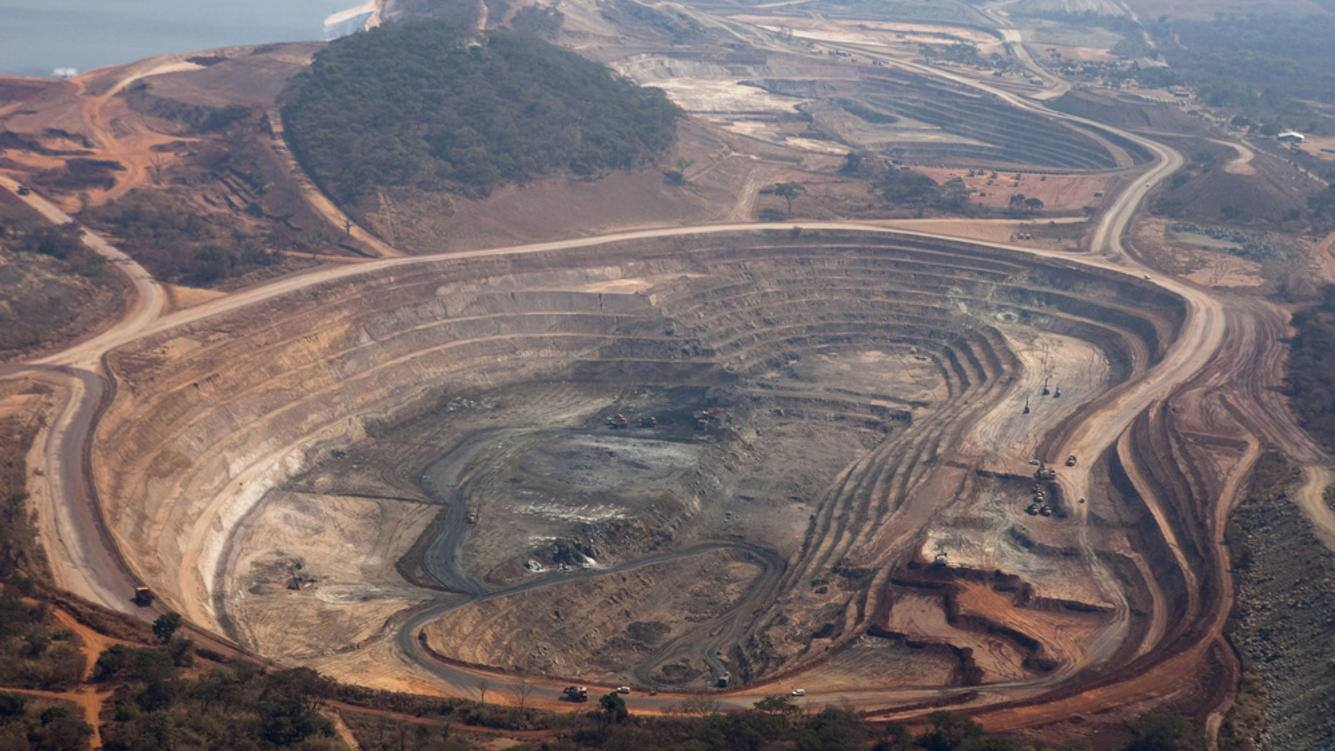
\includegraphics[height=6.5cm]{gfx/mutanda} % figure itself
   \caption{The Mutanda Mine in the DRC. Source: Bloomberg}
   \label{fig:mutanda}
\end{minipage}\hfill
\end{figure}

Cobalt has played an important role in homogeneous catalysis as far back as the 1930s, when the German chemist, Otto Roelen, developed the world's first industrial hydrosilylation process (the \textit{oxo synthesis}) at Oxo Chemie.\textsuperscript{\cite{hapke:2020}}

In biological systems, cobalt is an essential trace element, most notably as an integral component in all four forms of vitamin B$_{12}$.

Notably, the famous Fischer$-$Tropsch process---which converts syngas or watergas into liquid hydrocarbons---relies almost universally on heterogeneous cobalt as the chief catalyst metal and has done so since its inception in 1925. Besides this, presently there are endeavours to further capitalise on the catalytic talents of cobalt for water splitting and CO\textsubscript{2} reduction.\textsuperscript{\cite{wang:2016, gao:2016}}

\section{Oxidations}
  
\noindent Molecular oxygen (O$_2$) is an attractive oxidant for several reasons.\textsuperscript{\cite{gavriilidis:2016}} In production settings, however, oxidations are avoided wherever possible since they are associated with use of toxic metals, halogenated solvents, undesired byproducts and poor atom economy. Therefore, process chemists are severely limited by their choice of possible reagents which must be in the necessary (or higher) oxidation level. From this perspective, molecular oxygen is ideal, given its advantage towards the atom economy of a given oxidation reaction. There are two major chief drawbacks to the adoption of aerobic oxidations in large scale processes, most notably in the pharmaceutical industry: (i) using organic solvents in the presence of oxygen poses a risk to safety, and (ii) their is a lack of efficient catalysts with satisfactory activities and selectivities for such transformations.\textsuperscript{\cite{osterberg:2014}}

In pharmaceutical synthesis organic solvents are often necessary, particularly for ensuring complete solvation of reagents and catalysts, etc. Combining fuel/oxidiser mixtures under heating and increased pressure presents an obvious risk of ignition which is challenging to alleviate.\textsuperscript{\cite{lewis:1987}} Whilst there have been industry-sponsored studies on the flammability of organic solvent vapours,\textsuperscript{\cite{brooks:2007, zabetakis:1965}} there is a distinct lack of data on the safe operation of aerobic oxidations at temperatures and pressures conducive for pharmaceutical processes.\textsuperscript{\cite{osterberg:2014}}

The Amoco process (named after the now-defunct \textbf{Am}erican \textbf{O}il \textbf{Co}mpany) represents a catalytic success story for oxidation chemistry and catalysis. The process is the predominant method of generating terphthalic acid, which is an industrially significant precursor for condensation polymers, such as polyethylene terephthalate. Interestingly, the autooxidation of \textit{para}-xylene to terephthalic acid relies on a unique combination of two homogeneous catalysts and an additional bromide source, which acts as a promoter. The Co$-$Mn$-$Br catalyst system is very much the key to the success of the process, which introduces new catalyst pathways and increases the catalyst activity by 16 times, compared to a single cobalt catalyst.\textsuperscript{\cite{tomas:2013, brill:1960}}

Nitrous oxide (N$_2$O) gas is another attractive oxidant these days. Whereas oxidising with O$_2$ gas may be consumed in a reaction by incorporation into the substrate, N$_2$O gas has the advantage of being itself reduced, forming new---and very stable---N$_2$ gas molecules. Clearly a real benefit can be had over O$_2$ when it comes to achieving a favourable reaction entropy and providing a $-\Delta$G (negative Gibbs free energy change) for any given oxidation.

\section{C$-$C Single Bond Cleavage}

\noindent As mentioned in \autoref{ss:chemistryandcatalysis}, carbon--carbon cross-coupling chemistry has been a focal point in synthetic chemistry since the 1970s. The success of the Suzuki--Miyaura, Kumada, Negishi, Sonogashira, Hiyama, Heck, and Stille reactions are a remarkable testiment to the demand for practical C$-$C bond-forming methodologies, and to modern day chemists C$-$C bond formation is considered a straighforward synthetic strategy for building molecular complexity.

Over the past several decades, the challenge of C--H bond activations has been tackled independently by many groups and has led to many innovative novel publications. Notably, in 1993 Murai et al. reported a highly innovative means of C--H bond functionalisation using catalytic amounts of an organometallic ruthenium complex.\textsuperscript{\cite{murai:1993}} This reaction---considered to be a milestone in contemporary chemistry---demonstrated that the site-selective functionalisation of non-polar $\sigma$-bonds could be both highly practical and atom-economic in the scope of organic synthesis which has since become a well-established field of chemistry.\textsuperscript{\cite{crabtree:2017, labinger:2017, roque:2018}}

In addition to bond forming reactions, bond breaking can offer an alternative means of enhancing structural complexity into organic frameworks in ways that are not easily generated in any other way. Despite their pervasiveness in organic compounds, C$-$C single bond activations remain a real synthetic challenge.

The bond dissociation energy (BDE) of C$-$C, C$=$C, and C$\equiv$C bonds are $347-377$ kJ mol$^{-1}$, $~710$ kJ mol$^{-1}$, and $~960$ kJ mol$^{-1}$, respectively. One would expect, therefore, that C$-$C bonds are far more easily broken than C$=$C and C$\equiv$C bonds.

Oxidative addition of C$-$C bonds is difficult to achieve thermodynamically, as the strength of C$-$C bonds are far stronger than metal--carbon bonds. Substrates are typically more inclined towards C$-$C bond cleavage if they are high in cyclic strain, or if they can gain aromaticity and thus form products low in free energy.\textsuperscript{\cite{sattler:2010, crabtree:2019}} C$-$C single bonds are particularly unreactive when both carbon atoms are sp$^3$ hybridised; such an electron configuration is highly kinetically stable due to a combination of steric hindrance of nearby atoms (\eg, C--H bonds) and the directional nature of the sp\textit{\textsuperscript{n}} hybridised orbitals used in covalent bonding. Furthermore, much of organic synthesis takes advantage of the reactivity of (i) $\pi$-bonds (e.g., C$=$C, C$=$O, etc.), (ii) polarised $\sigma$-bonds (\eg, C--Br, C--Li, etc.), and (iii) lone pairs of electrons.\textsuperscript{\cite{murakami:2016}} Carbon$-$hydrogen and carbon$-$carbon $\sigma$-bonds---which are ubiquitous in the scaffold of organic compounds---are distinctly lacking all three of these basic prerequisites for desireable reactivity.

\begin{figure}
\centering
\begin{minipage}{\textwidth}
   \centering
   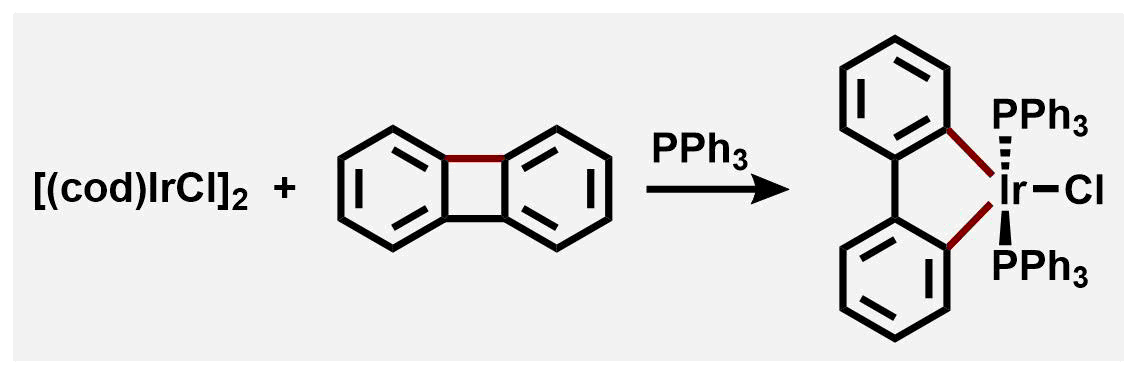
\includegraphics[height=3cm]{gfx/crabtree1} % figure itself
   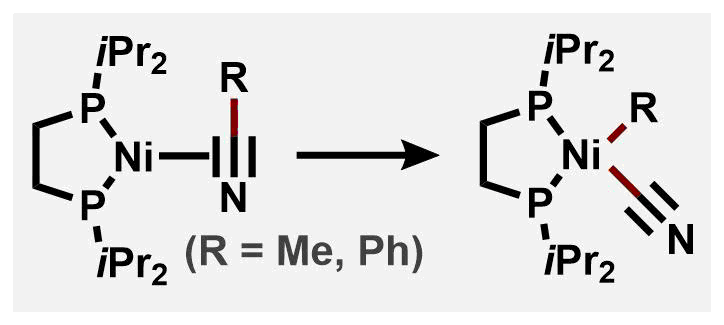
\includegraphics[height=3cm]{gfx/crabtree2} % figure itself
   \caption{Rare examples of C$-$C oxidative additions}
   \label{fig:crabtree}
\end{minipage}\hfill
\end{figure}

%\begin{figure}
%\centering
%\begin{minipage}{\textwidth}
%   \centering
%   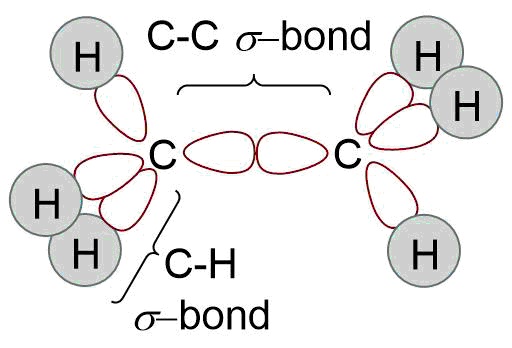
\includegraphics[height=3cm]{gfx/ethane} % figure itself
%   \caption{Ethane molecule: the simplest C(sp\textsuperscript{3})--C(sp\textsuperscript{3}) bond.}
%   \label{fig:ethane}
%\end{minipage}\hfill
%\end{figure}

\subsection{Applications}

C$-$C single bonds are broken routinely in industry where a long-chain hydrocarbon feedstock (such as naphtha) undergoes valorisation inside steam crackers. This energy-intense process is performed at high temperatures ($>$300$^{\circ}$C) to generate lighter hydrocarbons (typically olefins). Likewise, in the organic synthetic laboratory, C$-$C bond cleavage is well-documented using (over)-stoichiometric oxidants. Typical reagents include O$_3$,\textsuperscript{\cite{saliu:2012, suarez-bertoa:2012}} NaIO$_4$,\textsuperscript{\cite{binder:2008}} H$_5$IO$_6$, Pb(OAc)$_4$,\textsuperscript{\cite{criegee:1931}} and KMnO$_4$.

At the heart of many large chemical manufacturing plants is the steam cracker. This crucial piece of process technology provides the starting point for a value chains by taking crude oil fractions (typically naphtha) and "cracking" long chain saturated hydrocarbons into smaller unsaturated compounds, such as ethene and propene; these are the building blocks for myriad chemical comodities. The process for the cleavage of large hydrocarbons is facilitated by a heterogeneous catalyst---often zeolite-based---at temperatures of around 850$^{\circ}$C.

\subsection{Traditional Methods}

\noindent In 1931 Rudolf Criegee and co-workers first reported the cleavage of C(sp$^3$)$-$C(sp$^3$) bonds in vicinal diols (glycols), utilising Pb(OAc)$_4$ as an oxidant to generate aldehyde C(sp$^2$) centres on the two fragments.\textsuperscript{\cite{criegee:1931}} The Criegee oxidation works most effectively with diols glycols with hydroxy groups in close proximity.  \textit{cis}- and \textit{trans}-substituted diols may both proceed by forming a 5-membered cyclic intermediate with the lead atom. In the case of \textit{trans} substrates, a higher energy intermediate must be formed due to the relative orientation of the two oxygen atoms and high ring strain. The corresponding \textit{cis} intermediates are generated much more easily and more rapidly, therefore the reaction exhibits much greater selectivity towards \textit{cis} glycols. If the adoption of a highly strained 5-membered intermediate cannot be achieved, an alternative, slower, pathway is available.

In 1934 L\'eon Malaprade similarly reported a method for oxidative cleavage of C(sp$^3$)$-$C(sp$^3$) bonds in glycols but using hypervalent iodine reagent HIO$_4$ as an oxidant.\textsuperscript{\cite{malaprade:1934}} Due to the strong oxidising nature of HIO$_4$ the reaction may be viewed as less widely applicable that the Criegee oxidation, however, to its credit the Malaprade oxidation additionally provides an effective means of cleaving $\beta$-aminoalcohols.

\begin{figure}[hbt!]
\centering
\begin{minipage}{\textwidth}
   \centering
   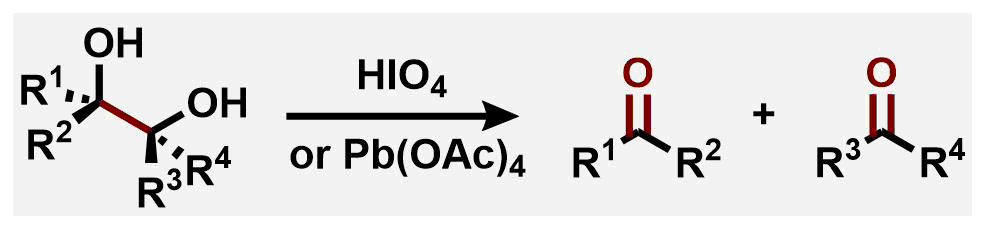
\includegraphics[height=2.2cm]{gfx/malaprade-criegee} % figure itself
   \caption{Criegee and Malaprade oxidations}
   \label{fig:malaprade-malaprade}
\end{minipage}\hfill
\end{figure}

\subsection{State-of-the-Art}

\noindent In recent years there C$-$C single bond activation reactions have come to the attention of chemists as a novel method for introducing valuable complexity within organic compounds. There are comparatively many reports of cleaving C$-$C bonds in there differently hybridised states,\textsuperscript{\cite{zhou:2015, qin:2016, liu:2017, liang:2017, zhao:2018, liu:2019, adeli:2019, tsang:2015}} however the cleavage of C(sp$^3$)$-$C(sp$^3$) bonds is far less reported.

Jiao and co-workers presented in 2017 a novel approach for the oxidative cleavage of allylic C(sp$^3$)$-$C(sp$^3$) bonds in the 

In 2018, Sarpong and co-workers reported a compelling \textit{deconstructive fluorination} methodology, which in a single step, cleaves a C(sp$^3$)$-$C(sp$^3$) bond and incorporates a new C$-$F bond in the process. Selectfluor (4 equiv) is used which acts as a fluorine donor to incorporate valuable complexity into an array of unstrained saturated \textit{N}-heterocycles, as shown in figure \ref{fig:sarpong1}.\textsuperscript{\cite{roque:2018}} Fluorine is widely used in the pharmaceutical and agrochemical industries for its so-called \textit{polar-hydrophobic} nature which can greatly impact lipophility, p\textit{K}\textsubscript{a}, and metabolic stability of small molecules.\textsuperscript{\cite{dalvi:2010}} Whilst this protocol describes the generation of interesting deconstructed products, it does rely on the use of overstoichiometric Selectfluor and AgBF$_4$ (4 equiv of both), and is poorly atom effiecient. Nevertheless, this innovative publication inspired many researchers to investigate the utility of activating C(sp$^3$)$-$C(sp$^3$) bonds for a fundamentally new approach to skeletal diversification. 

\begin{figure}[hbt!]
\centering
\begin{minipage}{\textwidth}
   \centering
   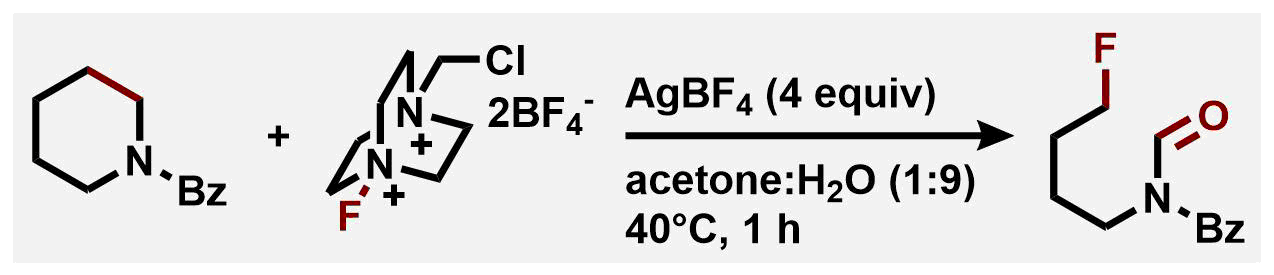
\includegraphics[height=2.5cm]{gfx/sarpong1} % figure itself
   \caption{Deconstructive fluorination using SelectFluor}
   \label{fig:sarpong1}
\end{minipage}\hfill
\end{figure}

The utilisation of lignin in chemistry is highly sought after; it is the main component of lignocellulosic biomass and it is the most ubiquitous renewable source of aromatic units known. Thus it has real potential to be a lucrative feedstock, especially since lignin is a waste product from the paper pulp industry. Phenol, a simple hydroxylated benzene ring, is a valued industrial commodity with a total annual production greater than $11.5$ megatons and is further processed to make dyes, polymers, pharmaceuticals and many other important products.\textsuperscript{\cite{morimoto:2015}} The chemical industry produces phenol from benzene in multistep synthesis under harsh conditions, consuming vast quantities of energy in the process. Naturally, benzene is derived from fossil resources and overall the industrial synthesis of phenol has raised environmental concerns. Achieving selectivity is challenging via this route, given that the hydroxylation of aromatic rings tends towards overoxidation.\textsuperscript{\cite{zhu:2019}} Valorisation of lignin thus presents an interesting, albeit challenging, alternative route towards the synthesis of aromatics such as phenol. Recently, Han and co-workers demonstrated just that, by using a solid acid catalyst and water to facilitate the cleavage of C$-$C single bonds (C(sp$^2$)$-$C(sp$^3$) hybridised) and C$-$O bonds within the complex polymeric material. This procedure was demonstrably effective upon scale-up whereby 4.1 g of phenol was obtained from 50.0 g of lignin.\textsuperscript{\cite{yan:2020}}

\section{Multivariate Optimisation}

\noindent Experimental design is a central concern in academia as well as in industrial chemistry. It is often a challenging endevour to establish fruitful reaction conditions with the optimal combination of reagents, solvents, catalysts, etc. for a reaction.

Univariate optimisation is an investigation of one-factor-at-a-time (OFAT) and is often limited by its small coverage of chemical space and its inability to detect how any interaction between variables may affect the reaction outcomes (\eg, yield, selectivity, etc.).

Reaction optimisation is often performed using a one-factor-at-a-time approach, whereby a scientist only considers a single variable's effect on the outcome of a reaction (\eg\ yield, selectivity, catalyst activity, etc.). Whilst this method can be useful, it is in fact inefficient and often lacking in accuracy. A multivariate analysis of variables on the other hand can be used to investigate a large volume of chemical space in an efficient and expedient manner with greater accuracy than a linear anaysis of variables.

OFAT optimisation rarely provides much insight into which factors are most influencial on the outcome of a reaction and provide no information about any interations between factors which are frequently present.

Design of Experiments (DoE) is a type of multivariate analysis that relies on statistics. In this way, no only can it be used to determine optimal reaction conditions, it also provides the advantage of quantifying the relative effect that each variable has on a reaction outcome. DoE is regularly employed in industry, however it is seldom used in academia despite its many advantages. Its increasingly favourable reputation and popularity amongst industrial chemists is a response to several key reasons:

\begin{enumerate}
  \item The development of high-throughput experimentation (HTE) using parallel reactors and flow reactor setups has become widely implemented.
  \item Quality by testing has largely been superseded by quality by design (QbD) and led to more widespread understanding of design space
  \item Green Chemistry Principles\textsuperscript{\cite{anastas:2010}} have encouraged chemists to reduce the waste output from chemical reactions and increase efficiency by reducing the amounts of solvents and reagents used in chemical processes
\end{enumerate}


Figures \ref{fig:doe-1} and \ref{fig:doe-2} compare the different optimum values obtained from univariate and multivariate analyses, and shows how the order in which factors are investigated will often impact the set of favourable reaction conditions revealed, \ie, the combination of conditions which furnish the most desireable outcome.

\begin{figure}
\centering
\begin{minipage}{0.45\textwidth}
   \centering
   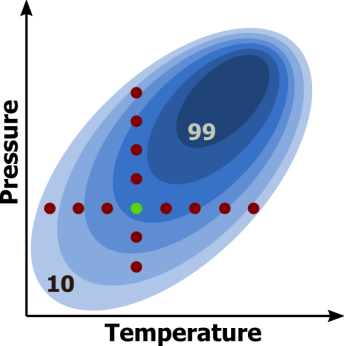
\includegraphics[height=5.4cm]{gfx/doe-1} % first figure itself
   \caption{OFAT study:\\two sequential studies, first exploring T, then \textit{p}}
   \label{fig:doe-1}
\end{minipage}\hfill
\begin{minipage}{0.45\textwidth}
   \centering
   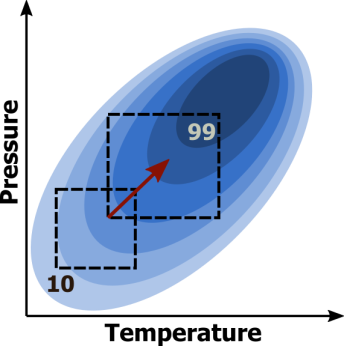
\includegraphics[height=5.4cm]{gfx/doe-2} % second figure itself
   \caption{Full-factorial study:\\one study exploring T and \textit{p} at the same time}
   \label{fig:doe-2}
\end{minipage}
\end{figure}

DoE can be used to investigate the effects of variables at several different numerical values. For this reason, for an effective DoE, it is valuable to have some prior knowledge about the reaction under investigation to select a suitable range of conditions to explore; if all reactions reach zero conversion then it is difficult to ascertain which factors are impeding the progress of the reaction. In other words, one should have at least a vague idea of suitable chemical space to explore.

The most common type of DoE is a \textit{factorial design}, which is represented as a \textit{base} raised to a \textit{power}. The \textit{number of levels} is given by the base, and the \textit{number of variables} is given by the power. Thus a $2^3$ design signifies a two-level three-factorial design. A design of this kind would therefore consist of $8$ experimental runs in addition to, perhaps, $4$ \textit{centre points}---additional experimental runs which are perfromed using the conditions in the very centre of the design space and allow for the reproducability of a reaction to be assessed, and provide a further data point in the optimisation---for a total of $12$ runs. In figure \ref{fig:doe-4} such a design is shown.

As the number of investigation varaiables increases, the number of experimental runs grows exponentially. For large numbers of variables this can be exceptionally demanding not only in terms of the cost of materials and equipment, but also with respect to time. 

\begin{figure}
\centering
\begin{minipage}{0.3\textwidth}
   \centering
   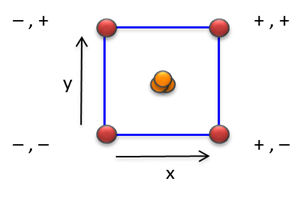
\includegraphics[height=3.2cm]{gfx/doe-3} % first figure itself
   \caption{$2^2$ design}
   \label{fig:doe-3}
\end{minipage}\hfill
\begin{minipage}{0.3\textwidth}
   \centering
   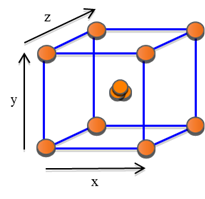
\includegraphics[height=3.2cm]{gfx/doe-4} % second figure itself
   \caption{$2^3$ design}
   \label{fig:doe-4}
\end{minipage}\hfill
\begin{minipage}{0.3\textwidth}
   \centering
   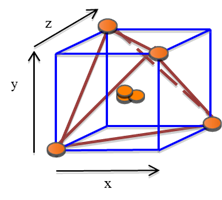
\includegraphics[height=3.2cm]{gfx/doe-5} % second figure itself
   \caption{$2^{3-1}$ design}
   \label{fig:doe-5}
\end{minipage}
\end{figure}

In 2002, Trevor Laird, at the time the editor of \textit{Organic Process Research \& Development} expressed his concerns regarding the reluctance of organic chemists to incorporate DoE techniques in their research, despite their efficacy in areas such as optimisation and for examining structure--activity relationships.\textsuperscript{\cite{laird:2002}}

% Papers to read: weissman:2015
% Diagram of univariate vs. multivariate
DoE has proven effective and gained popularity in industry as a practical tool for reaction optimisation and process improvements. This has been demonstrated by Pfizer with the simplified and cleaner synthesis of sertraline hydrochloride (Zoloft), a popular selective serotonin reuptake inhibitor, used to treat depression and anxiety-related disorders.\textsuperscript{\cite{taber:2004}}
